\documentclass[conference]{IEEEtran}
\usepackage{graphicx}
\usepackage{cite}
\usepackage{amsmath}
\usepackage[T1]{fontenc}
\usepackage{array}

\begin{document}

\title{Reproducing a Metric-Weighted CNN Ensemble for Pediatric Pneumonia Detection: A Like-for-Like Comparison and Failure Analysis}

\author{
\IEEEauthorblockN{Aman Kumar}
\IEEEauthorblockA{Roll no. 230065\\ Newton School of Technology, Rishihood University}\and
\IEEEauthorblockN{Asmit}
\IEEEauthorblockA{Roll no. 230063\\ Newton School of Technology, Rishihood University}\and
\IEEEauthorblockN{Shashwat}
\IEEEauthorblockA{Roll no. 230127\\ Newton School of Technology, Rishihood University}
}

\maketitle

\begin{abstract}
Deep learning papers on chest X-ray classification often report accuracies close to 99\%, but these numbers are rarely re-checked by an independent team. We reproduce the ensemble of Kundu et al. (PLOS ONE, 2021), which combines ImageNet-pretrained GoogLeNet, ResNet-18 and DenseNet-121 through a metric-based weighted average, on the 5,856-image Kermany pediatric chest X-ray dataset with five-fold cross-validation. Our ensemble reaches 98.72 $\pm$ 0.60\% accuracy, 99.11\% precision, 99.13\% recall and 99.12\% F1, all within 0.33 percentage points (pp) of the paper. A first comparison suggested that our AUC was 1.49 pp higher. Reading the official code showed that the paper computes AUC from hard predicted labels, which is the same as balanced accuracy. Measured the same way, our AUC is 98.37\% against the reported 98.35\%. Our failure analysis shows that (i) Normal images are misclassified about 2.8 times as often as Pneumonia images, (ii) the learned ensemble weights are almost exactly 1/3 each, so the weighting behaves like a plain average, (iii) the ensemble beats the best single backbone in only two of five folds, and (iv) every backbone reaches 100\% training accuracy by epoch 13 while validation loss stops improving. We also pre-registered one controlled change, Contrast Limited Adaptive Histogram Equalization (CLAHE), and implemented and tested the full experiment. It has not yet been run because of compute limits, so no CLAHE results are reported.
\end{abstract}

\begin{IEEEkeywords}
Pneumonia detection, chest X-ray, deep ensembles, transfer learning, reproducibility, CLAHE, failure analysis
\end{IEEEkeywords}

\section{Introduction}
Pneumonia is one of the leading causes of death in children under five. A chest X-ray is the most common imaging test used to diagnose it, but reading X-rays needs trained radiologists, who are scarce in many regions. Convolutional neural networks (CNNs) trained on public datasets now report accuracies close to 99\% on this task \cite{kermany,chexnet,kundu}.

A high number in a paper is only useful if someone else can obtain it again. Many machine-learning papers leave out details such as the random seed, the validation split or the exact metric code \cite{gundersen}, and a model that looks excellent on one dataset can fail on data from another hospital \cite{zech,roberts}. Our project therefore asks a simple question: \textit{if an independent student team re-implements a published pneumonia classifier, do they get the same numbers, and where does the model still fail?}

We chose Kundu \textit{et al.} \cite{kundu} as our base paper because it has public code, uses a public dataset, and combines three different CNNs with a simple, clearly defined weighting rule. Our contributions are:

\begin{itemize}
\item An independent, fully checkpointed five-fold reproduction of the Kundu ensemble on the Kermany dataset (5,856 images).
\item A like-for-like comparison with the paper. We show that an apparent 1.49 pp AUC gain disappears once AUC is computed the same way as in the official code.
\item A failure analysis of the reproduced system: class-wise errors, fold-to-fold variation, ensemble weights, and training dynamics.
\item A pre-registered, controlled CLAHE experiment that is fully implemented and tested. We report it as a planned experiment because it has not yet been run.
\end{itemize}

\section{Related Work}
Kermany \textit{et al.} \cite{kermany} released the pediatric chest X-ray dataset used here and showed that transfer learning from ImageNet \cite{imagenet} works well on it. CheXNet \cite{chexnet} trained a 121-layer DenseNet on the larger ChestX-ray14 dataset and compared it with radiologists. Several later works fine-tuned single pretrained CNNs on the Kermany data \cite{stephen,rahman}, and Chouhan \textit{et al.} \cite{chouhan} combined several pretrained networks into an ensemble. Kundu \textit{et al.} \cite{kundu} extended this idea with a weighted average whose weights come from each model's precision, recall, F1 and AUC.

Two strands of work motivate our analysis. Zech \textit{et al.} \cite{zech} showed that pneumonia models can learn hospital-specific shortcuts and lose accuracy on external data. Roberts \textit{et al.} \cite{roberts} reviewed hundreds of chest-imaging models and found frequent problems such as data leakage and unclear evaluation. On the image-processing side, adaptive histogram equalization \cite{pizer} and its contrast-limited version, CLAHE \cite{zuiderveld}, are standard ways to improve local contrast in medical images. This motivates our proposed change.

\section{Base Paper and Reproducibility Check}
Kundu \textit{et al.} fine-tune ImageNet-pretrained GoogLeNet \cite{googlenet}, ResNet-18 \cite{resnet} and DenseNet-121 \cite{densenet} for two classes and combine their class probabilities with the weight

\begin{equation}
w_i = \tanh(P_i) + \tanh(R_i) + \tanh(F1_i) + \tanh(\mathit{AUC}_i)
\end{equation}
where \textit{P}, \textit{R} and \textit{F1} are precision, recall and F1 score. The predicted class is the one with the highest weighted probability. On the Kermany dataset the paper reports 98.81 $\pm$ 0.61\% accuracy over five folds.

\textbf{Reproducibility checklist.} The paper and dataset are public, and the official repository provides the probability-extraction and ensembling code. Three details were missing or different, and we had to choose them ourselves: the fold seed, whether a validation split is used for checkpoint selection, and the learning-rate schedule. The paper's text and the code also differ slightly. Table I lists every difference.

\begin{table}[!t]
\caption{Differences between our protocol and the original}
\centering
\footnotesize
\setlength{\tabcolsep}{3pt}
\begin{tabular}{lcc}
\hline
\textbf{Item} & \textbf{Kundu et al.} & \textbf{Ours} \\
\hline
Fold seed & not stated & random\_state = 42 \\
Training images per fold & 4,686 & 4,216 (+469 validation) \\
Checkpoint choice & not stated & lowest validation loss \\
LR schedule (official code) & StepLR (10, 0.1) & ReduceLROnPlateau (0.1, 3) \\
GoogLeNet auxiliary heads & not stated & not trained \\
Ensemble weights from & training set & training part of each fold \\
Framework & PyTorch 1.9 & PyTorch 2.11, torchvision 0.26 \\
\hline
\end{tabular}
\end{table}

\section{Methods}
\subsection{Dataset}
We use the Kermany pediatric chest X-ray dataset \cite{kermany} from Kaggle. It contains 5,856 anterior-posterior X-rays of children aged one to five: 1,583 Normal and 4,273 Pneumonia, so Pneumonia images outnumber Normal ones by about 2.7 to 1. As in the base paper, we pool the official train and test folders and use stratified five-fold cross-validation with seed 42. In each fold, about 1,171 images (317 Normal, 854 Pneumonia) are held out for testing. Of the remaining 4,685 images, 10\% (469) form an internal validation set and 4,216 are used for training.

\begin{figure}[!t]
\centering
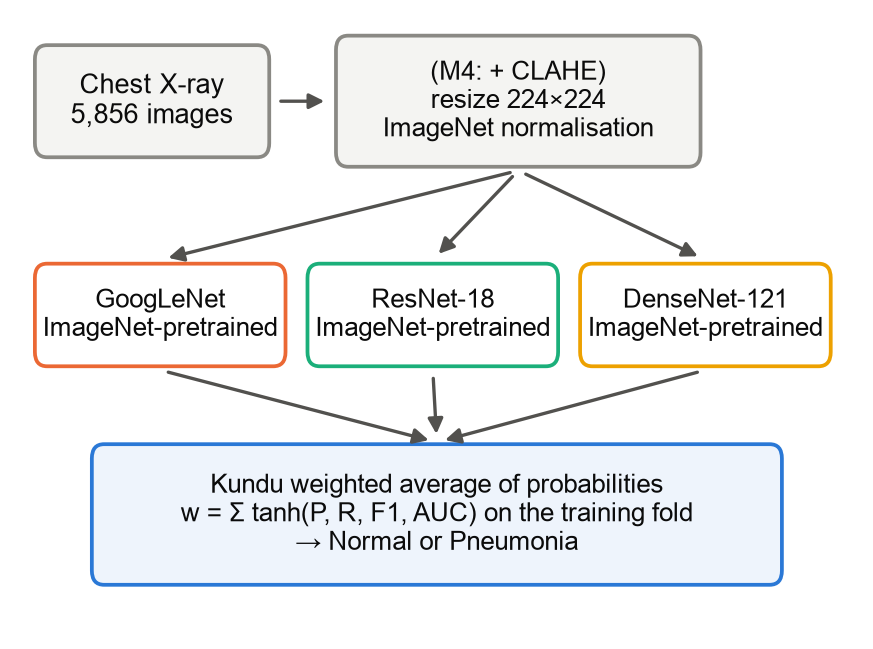
\includegraphics[width=\columnwidth]{fig/col_pipeline.png}
\caption{Reproduced pipeline. Each X-ray is resized and normalised, passed through three fine-tuned CNNs, and their probabilities are combined with Kundu's weights. The planned M4 change (CLAHE) would be added before the resize.}
\end{figure}

\subsection{Pre-processing and models}
Each image is converted to three channels, resized to 224 $\times$ 224 pixels and normalised with the ImageNet mean and standard deviation. No data augmentation is used, matching the official code. All three backbones start from ImageNet weights; their final layer is replaced by a two-class layer and all layers are fine-tuned (Fig. 1).

\subsection{Training}
Each model is trained for 30 epochs with Adam \cite{adam} (learning rate 10\textsuperscript{$-$4}), cross-entropy loss and batch size 16. The learning rate is reduced by a factor of 10 when the validation loss has not improved for more than three epochs, and we keep the weights with the lowest validation loss. Ensemble weights are computed from predictions on the training part of each fold, so the held-out fold is never used to choose anything. Because free Google Colab sessions disconnect often, our training code saves a checkpoint after every epoch and resumes from it automatically. This changes reliability, not results.

\subsection{Metrics}
We report accuracy, and precision, recall and F1 with Pneumonia as the positive class. We also report the recall of each class: \textit{Normal recall} (specificity) and \textit{Pneumonia recall} (sensitivity). AUC is reported in two ways. \textit{AUC-prob} is the standard area under the ROC curve computed from predicted probabilities. \textit{AUC-hard} is computed from hard 0/1 predictions, which mathematically equals the balanced accuracy, (Normal recall + Pneumonia recall)/2. Section VI explains why both are needed. All values are the mean $\pm$ standard deviation over the five held-out folds.

\section{Hypothesis and Planned Experiment}
\textbf{Hypothesis (submitted before coding).} Early pneumonia often appears as faint, low-contrast haze in the lungs. CLAHE \cite{zuiderveld} boosts contrast inside small tiles of the image and caps the boost to avoid amplifying noise. We predicted that adding CLAHE before the resize would \textit{increase} Pneumonia recall and AUC-prob, and would \textit{not decrease} F1. We also noted a risk: CLAHE can amplify noise, text labels and edge artefacts.

\textbf{Design.} Table II lists the experiments. CLAHE is the only change: the held-out images, internal validation split, seeds, optimiser, schedule and ensemble rule stay identical, so every comparison is paired fold by fold. The ablations ask whether any contrast boost works (global equalisation) and whether strength matters (clip limits 1, 2, 4). A run with no enhancement but the new seeds measures how much the metrics move from re-training alone. We planned paired t-tests over folds and an exact McNemar test \cite{mcnemar} over the 5,856 paired image-level predictions.

\begin{table}[!t]
\caption{Pre-registered CLAHE experiment (implemented, not yet executed)}
\centering
\footnotesize
\setlength{\tabcolsep}{3pt}
\begin{tabular}{lccc}
\hline
\textbf{ID} & \textbf{Change} & \textbf{Models} & \textbf{Question} \\
\hline
E1 & CLAHE, clip 2.0, 8$\times$8 & all 3 + ensemble & Does CLAHE help? (hypothesis) \\
E2a & Global hist. equal. & ResNet-18 & Is \textit{local} contrast the key? \\
E2b/c & CLAHE, clip 1.0 / 4.0 & ResNet-18 & Does strength matter? \\
E2d & No enhancement & ResNet-18 & Re-training noise floor \\
\hline
\end{tabular}
\end{table}

\textbf{Status.} The full experiment is implemented in our notebook and was tested end-to-end on a small synthetic dataset. These tests confirmed that, with no enhancement, the new pipeline produces the same input tensors as the baseline, and that a training run interrupted midway resumes to exactly the same weights. We estimate the experiment needs about 5 to 10 GPU-hours on a free Colab T4, and it has \textbf{not yet been executed} within our project time. We therefore report \textbf{no CLAHE results} and leave the hypothesis open.

\section{Results: Reproduction}
Table III and Fig. 2 show the five-fold results. The ensemble reaches 98.72 $\pm$ 0.60\% accuracy and 99.13 $\pm$ 0.41\% Pneumonia recall. Among single models, GoogLeNet is strongest (98.58\%) and DenseNet-121 is weakest (97.95\%). The standard deviations (0.4 to 1.0 pp) are larger than most differences between models.

\begin{table}[!t]
\caption{Five-fold results of each backbone and the Kundu ensemble (mean $\pm$ SD, \%)}
\centering
\footnotesize
\setlength{\tabcolsep}{3pt}
\begin{tabular}{lccccc}
\hline
\textbf{Model} & \textbf{Accuracy} & \textbf{Precision} & \textbf{Recall} & \textbf{F1} & \textbf{AUC-prob} \\
\hline
GoogLeNet & 98.58 $\pm$ 0.96 & 99.09 $\pm$ 0.56 & 98.97 $\pm$ 0.87 & 99.03 $\pm$ 0.66 & 99.78 $\pm$ 0.17 \\
ResNet-18 & 98.33 $\pm$ 0.73 & 98.94 $\pm$ 0.48 & 98.76 $\pm$ 0.53 & 98.85 $\pm$ 0.50 & 99.74 $\pm$ 0.16 \\
DenseNet-121 & 97.95 $\pm$ 0.76 & 98.65 $\pm$ 0.89 & 98.55 $\pm$ 0.92 & 98.59 $\pm$ 0.52 & 99.61 $\pm$ 0.17 \\
\textbf{Ensemble} & \textbf{98.72 $\pm$ 0.60} & \textbf{99.11 $\pm$ 0.49} & \textbf{99.13 $\pm$ 0.41} & \textbf{99.12 $\pm$ 0.41} & \textbf{99.84 $\pm$ 0.12} \\
\hline
\end{tabular}
\end{table}

\begin{figure}[!t]
\centering
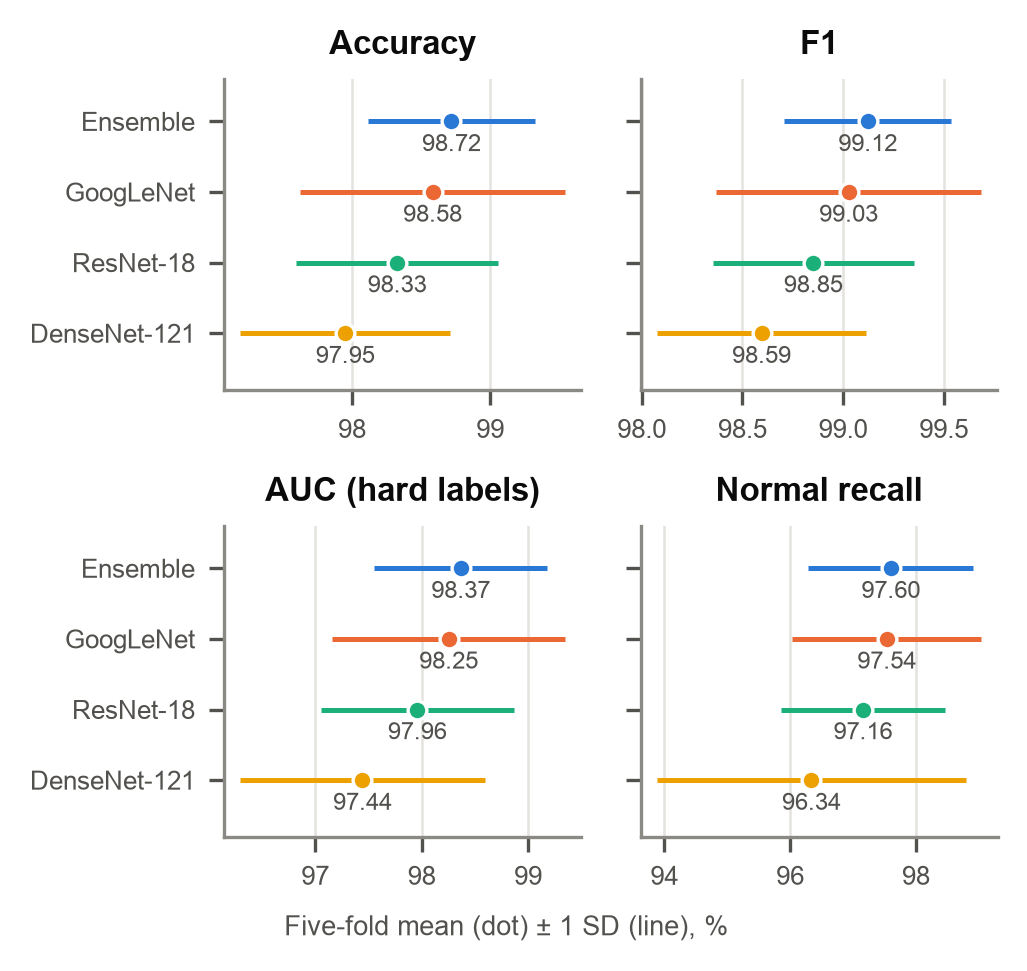
\includegraphics[width=\columnwidth]{fig/col_model_comparison.png}
\caption{Five-fold mean and standard deviation of each backbone and the ensemble. Note the different x-axis ranges; Normal recall is the lowest and most variable metric for every model.}
\end{figure}

\textbf{Comparison with the paper.} Our first comparison put our AUC 1.49 pp above the paper (99.84\% vs 98.35\%). The paper's AUC is lower than its own accuracy, which is unusual for a probability-based AUC, so we read the official code. It computes \texttt{roc\_auc\_score(labels, preds)} with \textit{hard predicted labels}, which yields balanced accuracy. Measured this way, our AUC is 98.37 $\pm$ 0.81\%, only 0.02 pp from the paper (Table IV, Fig. 3). Precision, recall and F1 use the same binary definitions in both works, so those comparisons were already fair. Every gap is smaller than one standard deviation, so we consider the reproduction successful.

\begin{table}[!t]
\caption{Comparison with Kundu et al. using the same metric definitions (mean $\pm$ SD, \%)}
\centering
\footnotesize
\setlength{\tabcolsep}{3pt}
\begin{tabular}{lccc}
\hline
\textbf{Metric} & \textbf{Kundu et al. \cite{kundu}} & \textbf{Ours} & \textbf{Gap (pp)} \\
\hline
Accuracy & 98.81 $\pm$ 0.61 & 98.72 $\pm$ 0.60 & $-$0.09 \\
Precision & 98.82 $\pm$ 0.59 & 99.11 $\pm$ 0.49 & +0.29 \\
Recall (sensitivity) & 98.80 $\pm$ 0.60 & 99.13 $\pm$ 0.41 & +0.33 \\
F1 & 98.79 $\pm$ 0.61 & 99.12 $\pm$ 0.41 & +0.33 \\
AUC, hard labels & 98.35 $\pm$ 0.68 & 98.37 $\pm$ 0.81 & +0.02 \\
AUC, probabilities & not reported & 99.84 $\pm$ 0.12 & --- \\
\hline
\end{tabular}
\end{table}

\begin{figure}[!t]
\centering
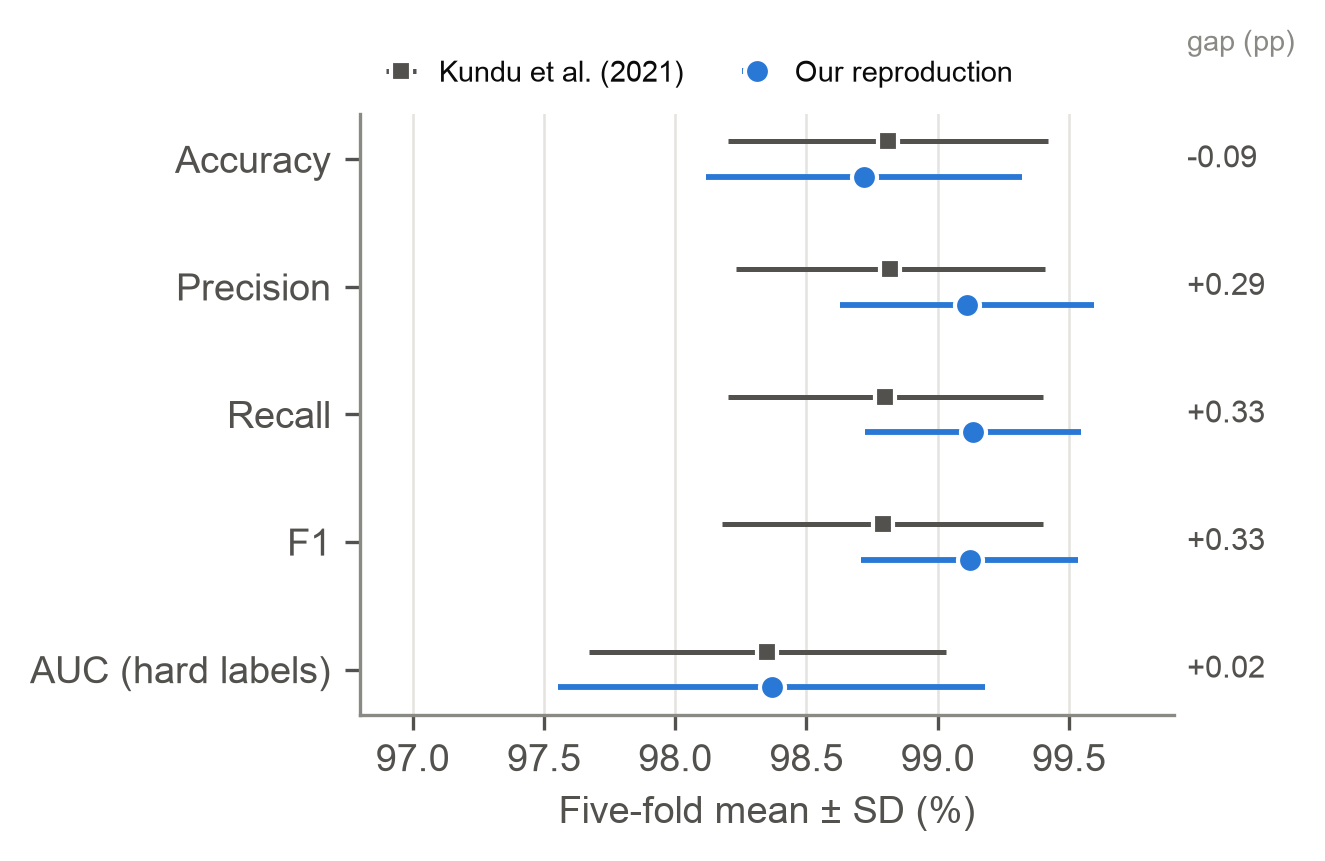
\includegraphics[width=\columnwidth]{fig/fig_kundu_comparison.png}
\caption{Kundu et al. vs our reproduction with matched metric definitions. Bars show $\pm$ 1 SD across folds; numbers on the right are mean gaps in percentage points.}
\end{figure}

\section{Failure Analysis}
\subsection{Which images does the ensemble get wrong?}
Pooling the five held-out folds gives 75 errors among 5,856 images (1.28\%): 38 Normal X-rays called Pneumonia (false positives) and 37 Pneumonia X-rays called Normal (false negatives) (Fig. 4). The raw counts look balanced, but the classes are not. Only 2.40\% of Normal images are wrong against 0.87\% of Pneumonia images, so \textbf{a Normal X-ray is about 2.8 times more likely to be misclassified}. The same pattern holds in every fold: Normal recall is 0.2 to 2.9 pp below Pneumonia recall (Fig. 5). The model sees 2.7 times more Pneumonia examples during training, and unweighted cross-entropy lets it lean toward the majority class. For a screening tool this is the safer direction, but it still means more healthy children would be sent for follow-up.

\begin{figure}[!t]
\centering
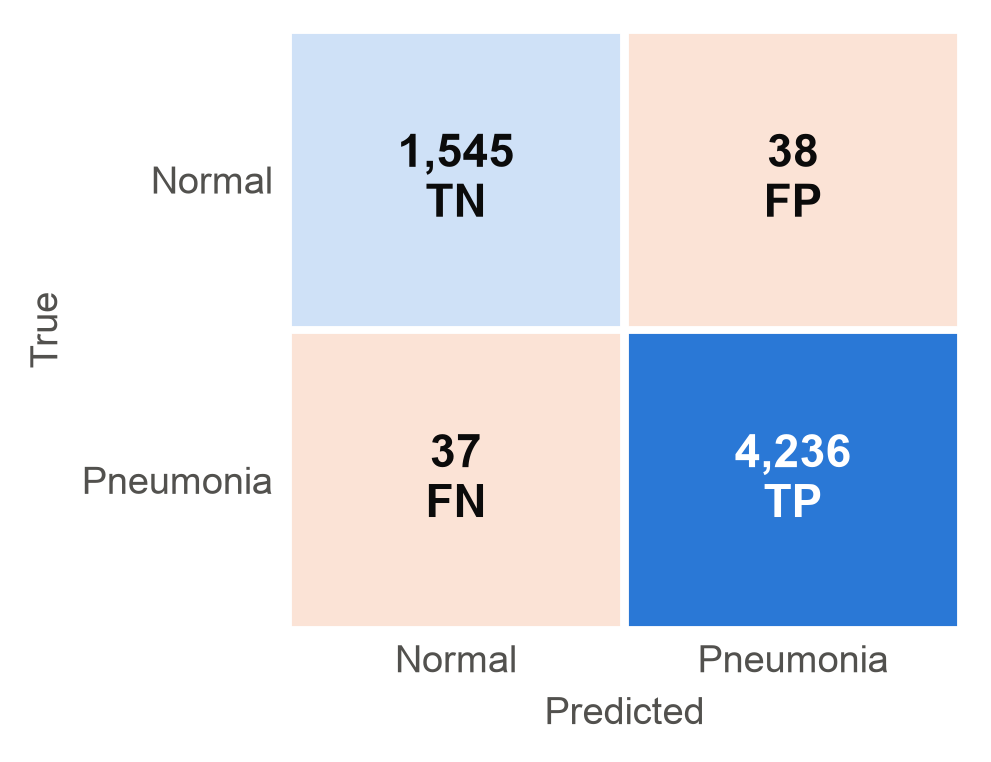
\includegraphics[width=\columnwidth]{fig/fig_confusion.png}
\caption{Pooled out-of-fold confusion matrix of the Kundu ensemble (5,856 images).}
\end{figure}

\begin{figure}[!t]
\centering
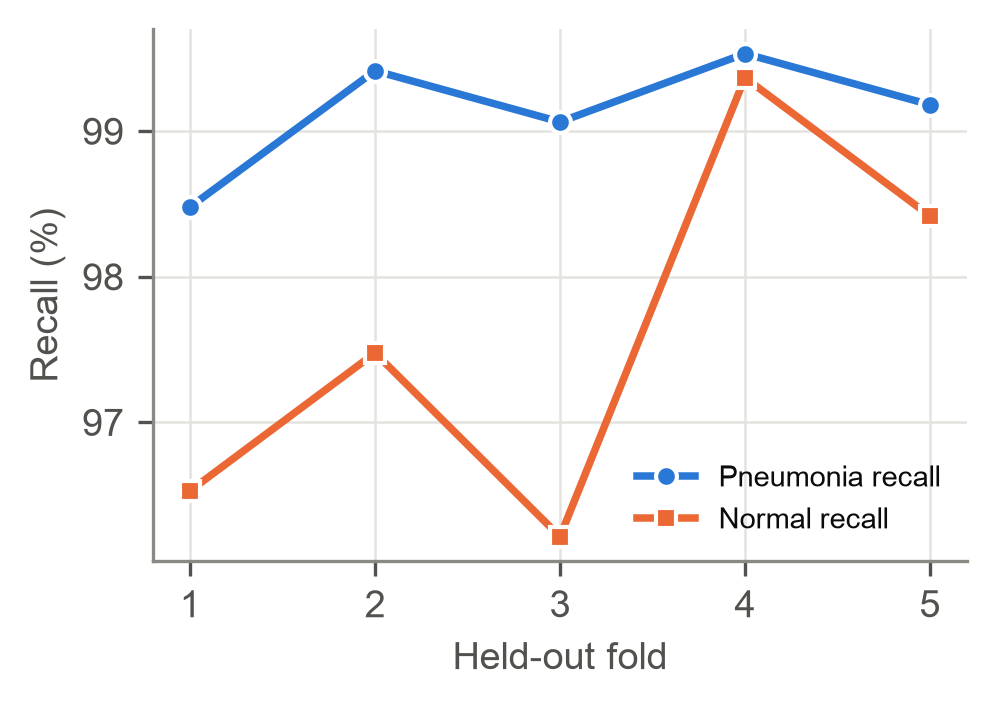
\includegraphics[width=\columnwidth]{fig/fig_class_recall.png}
\caption{Pneumonia recall vs Normal recall of the ensemble in each held-out fold.}
\end{figure}

\subsection{One fold is not enough}
Ensemble accuracy ranges from 97.95\% (fold 1) to 99.49\% (fold 4), a spread of 1.54 pp, which is 17 times the 0.09 pp gap to the paper (Fig. 6). Individual models vary even more. For example, DenseNet-121 flagged 24 of 317 healthy children in fold 2 (Normal recall 92.4\%) but only 5 in fold 5. A single train/test split could therefore make any of these models look best or worst.

\begin{figure}[!t]
\centering
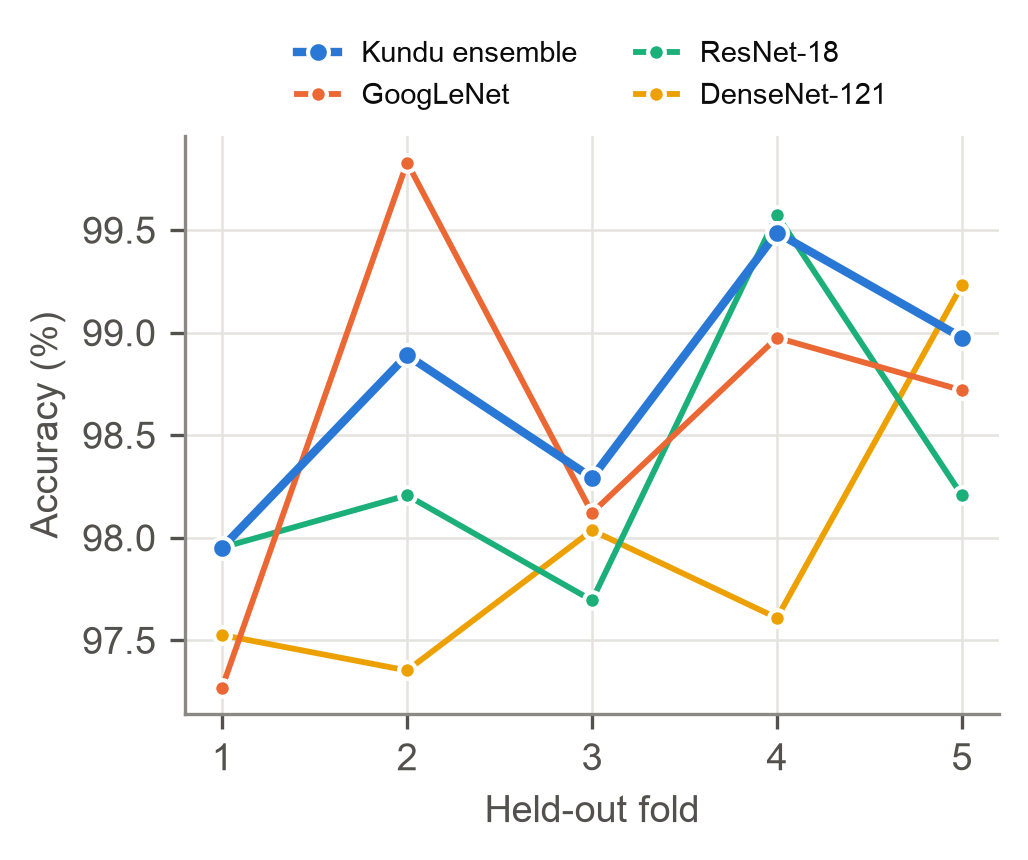
\includegraphics[width=\columnwidth]{fig/fig_per_fold_accuracy.png}
\caption{Accuracy of each model in each held-out fold. The ensemble is best or tied in only folds 1 and 3.}
\end{figure}

\subsection{Does the ensemble weighting help?}
The normalised Kundu weights were between 0.3327 and 0.3338 in every fold, practically 1/3 each. The weights are computed from training-fold predictions, and all three models reach almost 100\% training accuracy, so tanh of each metric is nearly identical. In practice the \textbf{weighted ensemble behaves like a plain average}. The ensemble's mean accuracy (98.72\%) is only 0.14 pp above GoogLeNet (98.58\%), and it beats the best single model in just two of five folds. In fold 2, GoogLeNet alone reached 99.83\% versus 98.89\% for the ensemble. Averaging mainly reduces variance (the ensemble has the smallest SD in most metrics) rather than raising the mean. Computing the weights on the internal validation split instead would give them a chance to differ.

\subsection{Training dynamics}
Our training logs cover seven complete runs (folds 3 to 5). In all of them, training accuracy reaches 100\% between epochs 9 and 13, while validation loss flattens early (Fig. 7). The plateau scheduler has reduced the learning rate to 10\textsuperscript{$-$6} or below by epochs 10 to 15, so the remaining 15 to 20 epochs barely change the weights. The best validation epoch varied from 3 to 22. In practice, about half of the training budget is spent on epochs that do almost nothing, which matters when GPU time is limited. Each epoch took 78 to 92 seconds for all three backbones even though their compute cost differs, which points to image loading on Colab's two CPU cores as the bottleneck. Our planned CLAHE pipeline therefore pre-computes and caches the resized images.

\begin{figure}[!t]
\centering
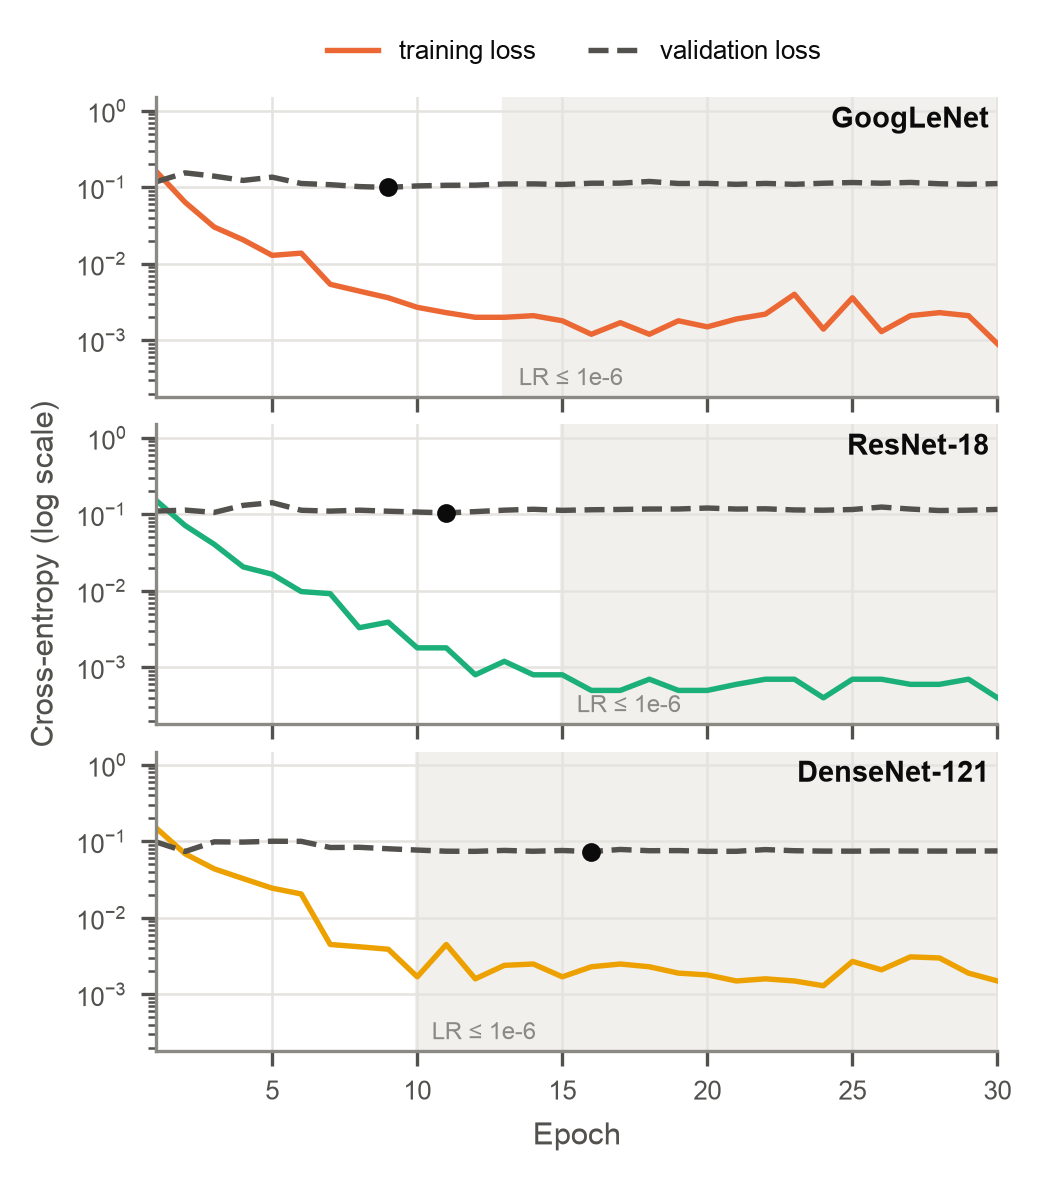
\includegraphics[width=\columnwidth]{fig/col_training_fold5.png}
\caption{Training and validation loss in fold 5. The shaded region is where the learning rate is at most 10\textsuperscript{$-$6}; the dot marks the selected (lowest validation loss) epoch.}
\end{figure}

\subsection{Metric definitions can create fake gains}
The AUC case in Section VI is itself a failure mode of comparing papers. Two numbers with the same name (AUC) measured different things, and the naive comparison suggested a 1.49 pp improvement that does not exist. We recommend that reproduction studies read the metric code, not only the paper text, and report a threshold-free AUC alongside any hard-label summary.

\section{Limitations and Future Work}
First, the planned CLAHE experiment has not been executed, so our hypothesis remains untested. Second, we use a single public dataset of young children from one hospital group, with no external test set, so the results say nothing about adults or other hospitals \cite{zech}. Third, like the base paper, we split by \textit{image} rather than by \textit{patient}. Kermany filenames encode a patient identifier, and some children have several X-rays, so images of the same child may appear in both training and test folds. This could inflate all reported scores \cite{roberts}. Our notebook includes a patient-leakage audit and a patient-grouped cross-validation run, a Grad-CAM attention check and a bacterial-versus-viral error breakdown, but we have not yet executed them and report no results from them. Finally, our training logs for folds 1 and 2 were not preserved in the notebook output, so the training-dynamics analysis uses folds 3 to 5. Future work is to run the CLAHE experiment and these analyses, compute ensemble weights on validation data, and test on an external dataset.

\section{Conclusion}
We independently reproduced the Kundu \textit{et al.} ensemble for pediatric pneumonia detection. With matched metric definitions, every metric lies within 0.33 pp of the paper and within one standard deviation. The apparent 1.49 pp AUC advantage came from a difference in how AUC was computed, not from a better model. Our failure analysis shows that the system is weaker on Normal X-rays than on Pneumonia X-rays, that its metric-based weights collapse to a plain average, and that fold-to-fold variation is much larger than the gap to the paper. These are research results on a public benchmark, not evidence of clinical readiness.

\begin{thebibliography}{99}
\bibitem{kermany} D. S. Kermany \textit{et al.}, ``Identifying medical diagnoses and treatable diseases by image-based deep learning,'' \textit{Cell}, vol. 172, no. 5, pp. 1122--1131, 2018.
\bibitem{chexnet} P. Rajpurkar \textit{et al.}, ``CheXNet: Radiologist-level pneumonia detection on chest X-rays with deep learning,'' arXiv:1711.05225, 2017.
\bibitem{kundu} R. Kundu, R. Das, Z. W. Geem, G.-T. Han, and R. Sarkar, ``Pneumonia detection in chest X-ray images using an ensemble of deep learning models,'' \textit{PLOS ONE}, vol. 16, no. 9, e0256630, 2021.
\bibitem{gundersen} O. E. Gundersen and S. Kjensmo, ``State of the art: Reproducibility in artificial intelligence,'' in \textit{Proc. AAAI Conf. Artificial Intelligence}, 2018, pp. 1644--1651.
\bibitem{zech} J. R. Zech \textit{et al.}, ``Variable generalization performance of a deep learning model to detect pneumonia in chest radiographs: A cross-sectional study,'' \textit{PLOS Medicine}, vol. 15, no. 11, e1002683, 2018.
\bibitem{roberts} M. Roberts \textit{et al.}, ``Common pitfalls and recommendations for using machine learning to detect and prognosticate for COVID-19 using chest radiographs and CT scans,'' \textit{Nature Machine Intelligence}, vol. 3, pp. 199--217, 2021.
\bibitem{imagenet} J. Deng \textit{et al.}, ``ImageNet: A large-scale hierarchical image database,'' in \textit{Proc. IEEE CVPR}, 2009, pp. 248--255.
\bibitem{stephen} O. Stephen, M. Sain, U. J. Maduh, and D.-U. Jeong, ``An efficient deep learning approach to pneumonia classification in healthcare,'' \textit{J. Healthcare Eng.}, vol. 2019, 4180949, 2019.
\bibitem{rahman} T. Rahman \textit{et al.}, ``Transfer learning with deep convolutional neural network (CNN) for pneumonia detection using chest X-ray,'' \textit{Applied Sciences}, vol. 10, no. 9, 3233, 2020.
\bibitem{chouhan} V. Chouhan \textit{et al.}, ``A novel transfer learning based approach for pneumonia detection in chest X-ray images,'' \textit{Applied Sciences}, vol. 10, no. 2, 559, 2020.
\bibitem{pizer} S. M. Pizer \textit{et al.}, ``Adaptive histogram equalization and its variations,'' \textit{Computer Vision, Graphics, and Image Processing}, vol. 39, no. 3, pp. 355--368, 1987.
\bibitem{zuiderveld} K. Zuiderveld, ``Contrast limited adaptive histogram equalization,'' in \textit{Graphics Gems IV}, P. S. Heckbert, Ed. San Diego, CA, USA: Academic Press, 1994, pp. 474--485.
\bibitem{googlenet} C. Szegedy \textit{et al.}, ``Going deeper with convolutions,'' in \textit{Proc. IEEE CVPR}, 2015, pp. 1--9.
\bibitem{resnet} K. He, X. Zhang, S. Ren, and J. Sun, ``Deep residual learning for image recognition,'' in \textit{Proc. IEEE CVPR}, 2016, pp. 770--778.
\bibitem{densenet} G. Huang, Z. Liu, L. van der Maaten, and K. Q. Weinberger, ``Densely connected convolutional networks,'' in \textit{Proc. IEEE CVPR}, 2017, pp. 4700--4708.
\bibitem{adam} D. P. Kingma and J. Ba, ``Adam: A method for stochastic optimization,'' in \textit{Proc. ICLR}, 2015.
\bibitem{mcnemar} Q. McNemar, ``Note on the sampling error of the difference between correlated proportions or percentages,'' \textit{Psychometrika}, vol. 12, no. 2, pp. 153--157, 1947.
\end{thebibliography}

\end{document}